\begin{pastexam}[label={px:gk3-100-ds-06}]{高考三級資訊處理 100 年 第六題}
（申論；10 分）

已知二元樹可以用一維陣列來儲存。請依此概念設計一方法，儲存以下三元樹於如下之一維陣列中。（10 分）
\begin{center}
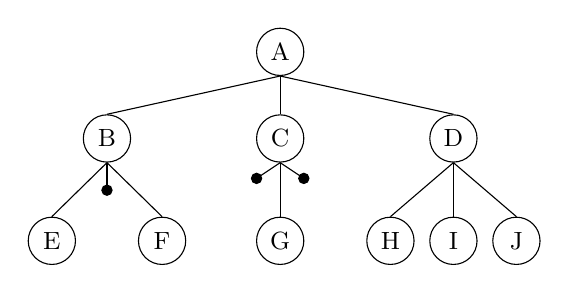
\begin{tikzpicture}[baseline=(A.base), every node/.style={circle,draw,minimum size=6mm,inner sep=0pt,font=\small},
  nul/.style={circle,fill,inner sep=0pt,minimum size=1.3mm}]
\node (A) at (0,0) {A};
\node (B) at (-2.2,-1.1) {B};
\node (C) at (0,-1.1) {C};
\node (D) at (2.2,-1.1) {D};
\node (E) at (-2.9,-2.4) {E};
\node (F) at (-1.5,-2.4) {F};
\node (G) at (0,-2.4) {G};
\node (H) at (1.4,-2.4) {H};
\node (I) at (2.2,-2.4) {I};
\node (J) at (3.0,-2.4) {J};
\draw (A.south) -- (B.north); \draw (A.south) -- (C.north); \draw (A.south) -- (D.north);
\draw (B.south) -- (E.north); \draw (B.south) -- (F.north);
\draw (B.south) -- ++(0,-0.35) node[nul] {};
\draw (C.south) -- (G.north);
\draw (C.south) -- ++(-0.3,-0.2) node[nul] {};
\draw (C.south) -- ++(0.3,-0.2) node[nul] {};
\draw (D.south) -- (H.north); \draw (D.south) -- (I.north); \draw (D.south) -- (J.north);
\end{tikzpicture}
\qquad
\begin{tabular}[t]{|l|l|l|l|l|l}
\hline
index & 0 & & & & \\ \hline
data & A & & & & \\ \hline
\end{tabular}
\end{center}
\end{pastexam}

\begin{pastsoln}
答案：根放在 index $0$，節點 $i$ 的三個子節點放在 $3i+1$、$3i+2$、$3i+3$，父節點在 $\lfloor (i-1)/3 \rfloor$。
\begin{center}
\begin{tabular}{|l|*{13}{c|}}
\hline
index & 0 & 1 & 2 & 3 & 4 & 5 & 6 & 7 & 8 & 9 & 10 & 11 & 12 \\ \hline
data & A & B & C & D & E & & F & & G & & H & I & J \\ \hline
\end{tabular}
\end{center}

\textbf{方法。} 二元樹用陣列存時，是把樹補成完整的二元樹，由上而下、由左而右依序編號；根在 $0$ 時
節點 $i$ 的子節點在 $2i+1$、$2i+2$（資結書第~7.2~節）。 三元樹照樣做：每個節點有左、中、右三個位置，
第 $d$ 層有 $3^{d}$ 個位置，逐層編號。 第 $i$ 個節點前面的每一個節點都佔用三個子位置，再加上根，
所以節點 $i$ 的第 $c$ 個子節點（$c = 1, 2, 3$）在
\[
3i + c,\qquad \text{父節點在 } \left\lfloor \frac{i - 1}{3} \right\rfloor \ (i \ge 1).
\]
空的子位置在陣列裡留空格（或填一個代表空的值）。

\textbf{放進陣列。} 圖中黑點是空的子位置：B 的中間子節點是空的，C 只有中間子節點 G。
\begin{itemize}
\item A 在 $0$，子節點在 $1, 2, 3$：B、C、D。
\item B（$1$）的子節點在 $4, 5, 6$：E、空、F。
\item C（$2$）的子節點在 $7, 8, 9$：空、G、空。
\item D（$3$）的子節點在 $10, 11, 12$：H、I、J。
\end{itemize}
共用 $13$ 格，其中 $3$ 格空著。 E、F、G、H、I、J 都是葉子，不必再往下留位置。 從陣列也能找回關係，
例如 G 在 $8$，父節點在 $\lfloor 7/3 \rfloor = 2$，就是 C，而 $8 = 3 \cdot 2 + 2$ 表示它是 C 的中間子節點。
\end{pastsoln}
